\documentclass[a4paper]{scrartcl}

\usepackage[utf8]{inputenc}
\usepackage[ngerman]{babel}
\usepackage{amsmath}
\usepackage{amssymb}
\usepackage{fancyhdr}
\usepackage{color}
\usepackage{graphicx}
\usepackage{lastpage}
\usepackage{listings}
\usepackage{tikz}
\usepackage{pdflscape}
\usepackage{subfigure}
\usepackage{float}
\usepackage{polynom}
\usepackage{hyperref}
\usepackage{tabularx}
\usepackage{forloop}
\usepackage{geometry}
\usepackage{listings}
\usepackage{fancybox}
\usepackage{tikz}
\usepackage{enumitem}
\usepackage{xcolor}

%Größe der Ränder setzen
\geometry{a4paper,left=3cm, right=3cm, top=3cm, bottom=3cm}

\fancyfoot[L]{}
\fancyfoot[C]{}
\fancyfoot[R]{Seite \thepage /\pageref*{LastPage}}

%Formatierung der Überschrift, hier nichts ändern
\def\header#1#2{
	\begin{center}
		{\Large Übungsblatt #1}\\
		{(Abgabetermin #2)}
	\end{center}
}

%Definition der Punktetabelle, hier nichts ändern
\newcounter{punktelistectr}
\newcounter{punkte}
\newcommand{\punkteliste}[2]{%
	\setcounter{punkte}{#2}%
	\addtocounter{punkte}{-#1}%
	\stepcounter{punkte}%<-- also punkte = m-n+1 = Anzahl Spalten[1]
	\begin{center}%
		\begin{tabularx}{\linewidth}[]{@{}*{\thepunkte}{>{\centering\arraybackslash} X|}@{}>{\centering\arraybackslash}X}
			\forloop{punktelistectr}{#1}{\value{punktelistectr} < #2 } %
			{%
				\thepunktelistectr &
			}
			#2 &  $\Sigma$ \\
			\hline
			\forloop{punktelistectr}{#1}{\value{punktelistectr} < #2 } %
			{%
				&
			} &\\
			\forloop{punktelistectr}{#1}{\value{punktelistectr} < #2 } %
			{%
				&
			} &\\
		\end{tabularx}
	\end{center}
}

\definecolor{lightgreen}{rgb}{0.55, 0.71, 0.0}
\definecolor{darkgreen}{rgb}{0.0, 0.5, 0.0}

\begin{document}
	
\section*{Wechseln zu IEC-Gatter-Symbolen}

\textbf{Bitte auf jeden Fall für Abgaben umstellen!} \\
Unter \textit{Datei $>$ Voreinstellungen...} im Reiter \textit{Internationalisierung $>$ Gatterform} \textbf{IEC (rechteckig)} auswählen. 

\subsection*{Zoom-Funktion}
	Unten Links findet sich die Funktion sie Skallierung hoch und runter zu stellen. 

\section*{Die Menüleiste}
	\begin{figure}[H]
		\centering
		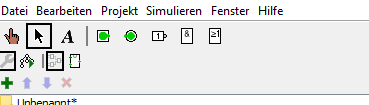
\includegraphics[]{Gatter.png}
	\end{figure}

	\begin{description}
		\item[Mauszeiger:] Modus fürs Bearbeiten des Schaltplans
		\item[Handsymbol:] Modus fürs Interagieren mit den Gattern (z.B. Takt umschalten, Tester drücken,...)
		\item[Das A-Symbol:] Fügt Texte dem Schaltnetz hinzu
		\item[Ordner mit Gatter:] Alle Bauteile in Kategorien eingeteilt (einfach mal durchklicken und schauen was es alles gibt)
	\end{description}

\section*{Gatter}
	\begin{figure}[H]
		\centering
		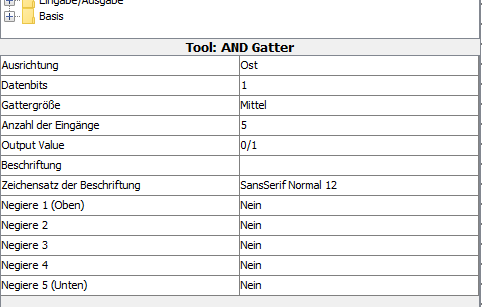
\includegraphics[height=7cm]{Gatter2.png}
	\end{figure}
	
	Nachdem ein Gatter ausgewählt wurde, öffnet sich die Eigenschaften des Gatters an der linken Seite.
	
	\begin{description}
		\item[Ausrichtung:] Ändert die Richtung in der der Ausgang zeigt
		\item[Anzahl der Eingänge:] Ändert die Anzahl an Eingänge des Gatters
		\item[Beschriftung:] Beschriftung des Gatters im Schaltnetz
	\end{description}


\section*{Schaltnetzaufbau}
	Modus: \textbf{Mauszeiger} \\
	Das im linken Bereich ausgewählte Bauteil kann im Raster rechts platziert werden. \\
	Hält man an einer Verbindung oder einem Gatterein-/ausgang die Maus gedrückt kann man von dort eine Verbindung ziehen. Dabei gilt \textcolor{lightgreen}{hellgrüne} Linien sind aktiv (logisch 1), \textcolor{darkgreen}{dunkelgrüne} auf tief (logisch 0), \textcolor{blue}{blaue} werden nicht verwendet und ignoriert und \textcolor{red}{rote} sind fehlerhaft oder müssen mit einem Wert belegt werden. \\
	Schaltnetze werden für gewöhnlich in Stages aufgeteilt, wobei die Gatter einer Stage in einer vertikalen Linie angeordnet werden. Zum Beispiel eine Stage in der alle Eingangsvariablen zusätzlich negiert werden, eine für die ersten Konjunktionen, ...\\
	\textit{Tipp:} Für Eingabevariablen sind Takte zu empfehlen (siehe Simulieren).
	
	\begin{figure}[H]
		\centering
		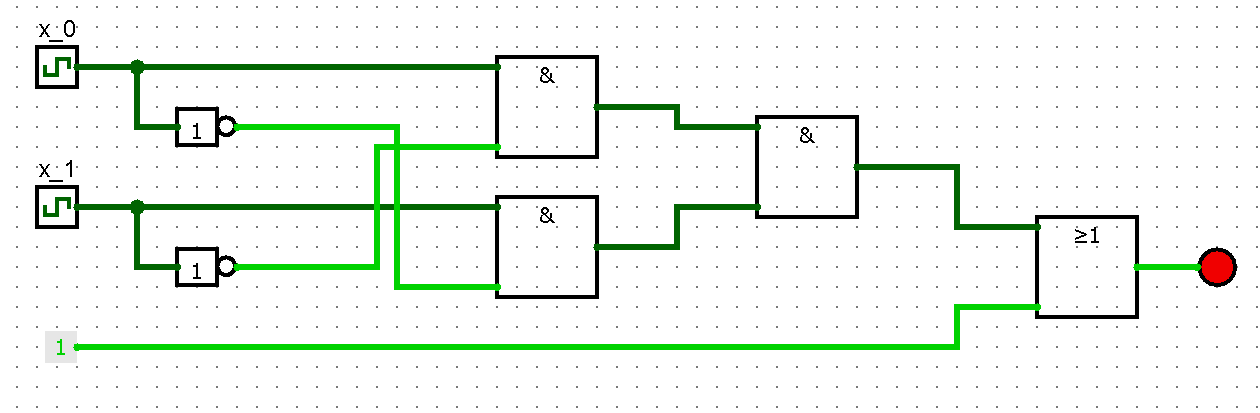
\includegraphics[width=\textwidth]{Tautologie.png}
		\caption{Beispiel von Stages einer Tautologie}
	\end{figure} 
	

\section*{Simulieren}

	Einzelne Eingabewechsel können mit der Hand überprüft werden. \\
	Bei zyklischen Schaltungen macht es Sinn automatisch durchzuschalten.
	Dazu müssen die Eingangsvariablen als Takte realisiert sein. In den Eigenschaften müssen entsprechend der \glqq Höhe\grqq des Bits die Taktlänge der High- \textbf{UND} Low-Pegels gesetzt werden. \\
	Im Beispiel wurde der Takt des most significant Bits $x_3$ auf $2^3 = 8$ Takten, $x_2$ auf 4, $x_1$ auf 2 und $x_0$ auf 1 Takt gesetzt.
	\begin{figure}[H]
		\centering
		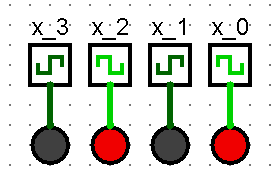
\includegraphics[]{Simulation.png}
	\end{figure} 
	
	Anschließend kann man mit folgenden Tastenkombinationen die Schaltung simulieren: \\
	\begin{description}
		\item[Strg + R] Setzt die Takte wieder auf den Anfang zurück (evtl. muss man auch das Programm neu starten)
		\item[Strg + T] Schaltet einen Takt weiter
		\item[Strg + K] Lässt die im Takt automatisch weiter laufen
		\item[Weitere Optionen] finden sich oben unter dem Reiter \textit{Simulation}
	\end{description}
	
\end{document}
%%% Local Variables:
%%% mode: latex
%%% TeX-master: t
%%% End:
